\documentclass[11pt,a4paper]{article}

% ── Core packages ──
\usepackage[margin=2.5cm]{geometry}
\usepackage[utf8]{inputenc}
\usepackage[T1]{fontenc}
\usepackage{graphicx}
\usepackage[colorlinks=true, linkcolor=blue, urlcolor=blue, citecolor=blue]{hyperref}
\usepackage[table]{xcolor}
\usepackage{colortbl}
\usepackage{booktabs}
\usepackage{tabularx}
\usepackage{float}
\usepackage{enumitem}
\usepackage{longtable}
\usepackage{amsmath, amssymb}
\usepackage[most]{tcolorbox}
\usepackage{titlesec}
\usepackage{fancyhdr}
\usepackage{caption}
\usepackage{subcaption}
\usepackage{multirow}
\usepackage{array}
\usepackage{pdflscape}
\usepackage{afterpage}

% ── Global list compaction ──
\setlist[itemize]{nosep, leftmargin=*, topsep=2pt, partopsep=0pt}
\setlist[enumerate]{nosep, leftmargin=*, topsep=2pt, partopsep=0pt}

% ── Widow/orphan control ──
\widowpenalty=10000
\clubpenalty=10000

% ── Page style ──
\pagestyle{fancy}
\fancyhf{}
\fancyhead[L]{\small\textit{Threshold-Based Unknown Species Detection}}
\fancyhead[R]{\small Experiment Report --- June 2026}
\fancyfoot[C]{\thepage}
\renewcommand{\headrulewidth}{0.4pt}

% ── Section formatting ──
\titleformat{\section}{\Large\bfseries}{\thesection}{1em}{}
\titleformat{\subsection}{\large\bfseries}{\thesubsection}{1em}{}

% ── Custom commands ──
\newcommand{\formula}[1]{\texttt{#1}}
\newcommand{\algo}[1]{\textsf{#1}}
\newcommand{\metric}[1]{\textbf{#1}}
\newcommand{\bestf}{0.4461}

\begin{document}

% ═══════════════════════════════════════════════════════════════
% TITLE PAGE
% ═══════════════════════════════════════════════════════════════

\begin{titlepage}
\centering
\vspace*{4cm}

{\Huge\bfseries Threshold-Based Unknown Species\\[8pt] Detection --- Full Experiment Report\par}

\vspace{1.5cm}

{\Large Experiment ID: \texttt{threshold-full-001}\par}

\vspace{1cm}

{\large June 2026\par}

\vspace{1.5cm}

{\normalsize
\textbf{Experiment Category:} Autoresearch --- Retrieval Threshold Optimization\\
\textbf{Repository:} MycoAI Monorepo --- \texttt{research/src/experiments/threshold/}\\
\textbf{Test Data:} 471 known (7 species, 15 test strains) $+$ 1{,}173 unknown (41 species, 50 strains)\\
\textbf{Formulas Evaluated:} 162 unique formulas $\times$ 3 algorithms $=$ 528 experiments
\par}

\vspace{2cm}

{\small
\begin{tcolorbox}[width=0.85\textwidth, colback=blue!5, colframe=blue!60, title={\textbf{Key Finding}}, fonttitle=\bfseries, center]
Best result: \formula{gap01\_sq} $+$ \algo{f1\_grid} achieves F1 $=$ \bestf{} (Precision $=$ 0.2876, Recall $=$ 0.9936, Specificity $=$ 0.0119).\\
Severe class imbalance dominates: the model labels nearly everything as ``known,'' yielding high recall but near-zero specificity. F1 alone is misleading for this task.
\end{tcolorbox}
}

\vfill
\end{titlepage}

% ═══════════════════════════════════════════════════════════════
% EXECUTIVE SUMMARY
% ═══════════════════════════════════════════════════════════════

\section{Executive Summary}

\subsection{Objective}

This experiment evaluates whether a score-based thresholding pipeline can reliably separate \textbf{known} fungal species (present in the training index) from \textbf{unknown} species (novel to the system). For each query image, a KNN retrieval returns the top-$K$ neighbours with similarity scores $(s_0, s_1, \ldots, s_4)$. A \emph{formula} maps these five scores to a scalar confidence value; a threshold applied to this value classifies the image as known ($\geq t$) or unknown ($<t$). The goal is to find the formula--algorithm--threshold combination that maximises the F1 score for the known class.

\subsection{Configuration}

The retrieval pipeline uses an EfficientNetB1 model fine-tuned on fungal colony features, querying the \texttt{myco\_fungi\_features\_full\_finetuned} Qdrant collection with $K=11$ neighbours under environment strategy E1 (same growth medium only) and weighted score aggregation.

\subsection{Test Data}

The test set comprises \textbf{471 known samples} drawn from 7 Penicillium species held out from the Qdrant index during retrieval (15 test strains across 7 growth environments) and \textbf{1{,}173 unknown samples} from 41 diverse fungal species (50 strains) never seen during training.

\subsection{Best Result}

The \formula{gap01\_sq} formula (squared difference between top-1 and top-2 scores) paired with the \algo{f1\_grid} threshold-finding algorithm yields F1 $=$ \bestf{} at threshold $t = 4.62 \times 10^{-7}$. This configuration correctly accepts 468 of 471 known samples (recall $=$ 99.4\%) but incorrectly accepts 1{,}159 of 1{,}173 unknown samples as known (specificity $=$ 1.2\%).

\subsection{Limitation}

F1 proves misleading as a primary metric for this task. The severe class imbalance (1,173 unknowns vs.\ 471 knowns) means that a strategy maximising F1 under standard grid search will always favour near-universal acceptance --- because recall dominates the F1 numerator when the threshold is set near zero. The result is a classifier with $>$99\% recall but effectively no ability to reject unknowns. Future work must incorporate false-positive-rate constraints, weighted loss functions, or a two-stage classification architecture.

% ═══════════════════════════════════════════════════════════════
% EXPERIMENT SETUP
% ═══════════════════════════════════════════════════════════════

\section{Experiment Setup}

\subsection{Retrieval Pipeline}

\begin{figure}[htbp]
\centering
\begin{tcolorbox}[width=0.95\textwidth, colback=gray!5, colframe=gray!40, title={\textbf{Retrieval Pipeline Architecture}}, fonttitle=\bfseries]
\begin{center}
Query Image $\rightarrow$ \textbf{EfficientNetB1\_finetuned} $\rightarrow$ Feature Vector $\rightarrow$ \\
\textbf{Qdrant} (\texttt{myco\_fungi\_features\_full\_finetuned}) $\rightarrow$ Top-$K$ Neighbours \\
$\rightarrow$ Score Vector $(s_0, s_1, s_2, s_3, s_4)$ $\rightarrow$ \textbf{Formula} $f(s_0, \ldots, s_4) \rightarrow$ Score \\
$\rightarrow$ \textbf{Threshold} $t$ $\rightarrow$ Known / Unknown Decision
\end{center}
\end{tcolorbox}
\caption{End-to-end retrieval and thresholding pipeline. The formula maps neighbour scores to a scalar; the threshold determines the known/unknown classification.}
\label{fig:pipeline}
\end{figure}

\noindent The retrieval configuration is fixed across all experiments:

\begin{tcolorbox}[colback=blue!3, colframe=blue!30, title={\textbf{Fixed Retrieval Parameters}}, fonttitle=\bfseries]
\begin{tabular}{@{}lll@{}}
\toprule
\textbf{Parameter} & \textbf{Value} & \textbf{Description} \\
\midrule
Collection & \texttt{myco\_fungi\_features\_full\_finetuned} & Qdrant vector store \\
Extractor & EfficientNetB1\_finetuned & Feature extractor backbone \\
$K$ & 11 & Top neighbours retrieved \\
Environment & E1 & Same growth medium only \\
Aggregation & Weighted & Score-weighted neighbour voting \\
\bottomrule
\end{tabular}
\end{tcolorbox}

\subsection{Test/Train Split}

The Qdrant index contains embeddings for 53 known Penicillium species (the curated dataset). Seven species were \textbf{held out} from the index during retrieval to serve as \emph{known} test samples, while the remaining 46 species constitute the training corpus. Additionally, 41 \emph{unknown} species from the incoming (diverse) dataset --- species entirely absent from the curated collection --- were retrieved against the index.

\subsection{Dataset Statistics}

\begin{table}[htbp]
\centering
\caption{Dataset composition for threshold experiment. Known samples span 7 species with 15 strains tested across 7 growth environments. Unknown samples span 41 species across 50 strains and 8 environments.}
\label{tab:dataset}
\begin{tabular}{@{}lrrr@{}}
\toprule
\textbf{Statistic} & \textbf{Known} & \textbf{Unknown} & \textbf{Total} \\
\midrule
Samples & 471 & 1{,}173 & 1{,}644 \\
Unique species & 7 & 41 & 48 \\
Unique strains & 15 & 50 & 65 \\
Growth environments & 7 & 8 & 8 \\
Images per species (mean) & 67.3 & 28.6 & 34.3 \\
\bottomrule
\end{tabular}
\end{table}

\noindent The known species and their sample counts are: \textit{P. freii} (102), \textit{P. polonicum} (99), \textit{P. melanoconidium} (54), \textit{P. viridicatum} (42), \textit{P. tricolor} (78), \textit{P. neoechinulatum} (54), and \textit{P. aurantiogriseum} (42). The growth environments span CYA (84), MEA (84), CREA (78), YES (72), DG18 (69), CYA30 (42), and CYAS (42).

The unknown dataset is more diverse but shallower per species. The five most frequent unknown species are \textit{P. nalgiovense} (90 samples), \textit{E. crustaceum} (69), \textit{P. expansum} (63), \textit{P. griseofulvum} (60), and \textit{E. egyptiacum} (36). Among environments, CYA and MEA dominate (276 and 270 samples respectively).

\subsection{Formula Design Space}

A \textbf{formula} is a function $f(s_0, s_1, s_2, s_3, s_4) \rightarrow \mathbb{R}$ that maps the five neighbour similarity scores to a single scalar confidence value. The design space explored 162 distinct formulas grouped into qualitative families:

\begin{table}[htbp]
\centering
\caption{Formula families and their naming conventions. Each family represents a qualitatively distinct mathematical transformation of the neighbour score vector.}
\label{tab:formulas}
\begin{tabular}{@{}llp{6.5cm}@{}}
\toprule
\textbf{Prefix} & \textbf{Count} & \textbf{Description} \\
\midrule
\formula{gap\_\{i\}\_\{j\}} & 10 & Score differences $s_i - s_j$ \\
\formula{gnorm\_\{i\}\_\{j\}} & 10 & Normalised gaps $(s_i - s_j)/(s_i + s_j)$ \\
\formula{ratio\_\{i\}\_\{j\}} & 20 & Score ratios $s_i / s_j$ \\
\formula{prod\_\{i\}\_\{j\}} & 10 & Score products $s_i \times s_j$ \\
\formula{avg\_top\{k\}} & 4 & Arithmetic mean of top-$k$ \\
\formula{gm\_top\{k\}} & 4 & Geometric mean of top-$k$ \\
\formula{hm\_top\{k\}} & 4 & Harmonic mean of top-$k$ \\
\formula{ne\_top\{k\}} & 4 & Normalised entropy of top-$k$ \\
\formula{std\_top\{k\}} & 4 & Standard deviation of top-$k$ \\
\formula{range\_top\{k\}} & 4 & Range of top-$k$ \\
\formula{exp\_decay\{N\}} & 4 & Exponentially weighted sum \\
\formula{w\_\{name\}} & 12 & Custom weight vectors \\
\formula{s\{i\}\_sq/sqrt/log} & 15 & Single-score power transforms \\
\formula{hyb\_\{type\}\_a\{N\}} & 4 & Hybrid gap-mean combinations \\
\formula{agree\_top\{k\}} & 2 & Inverse variance agreement \\
\formula{rat**\_p/m/x\_rat**} & 12 & Multi-term ratio chains \\
\formula{gnorm\_*\_x/p\_gnorm\_*} & 5 & Gnorm products and sums \\
\formula{wtd\_rat\_\{type\}} & 3 & Weighted ratio chains \\
\formula{s\{i\}\_rel\_\{stat\}} & 3 & s0-relative metrics \\
Other & 30 & Squared gaps, CV, reciprocal ratios, spread, log-ratios, etc. \\
\midrule
\textbf{Total} & \textbf{162} & \\
\bottomrule
\end{tabular}
\end{table}

\subsection{Threshold-Finding Algorithms}

Three algorithms determine the optimal threshold for each formula:

\begin{tcolorbox}[colback=green!3, colframe=green!30, title={\textbf{Algorithm Descriptions}}, fonttitle=\bfseries]
\begin{itemize}
  \item \algo{f1\_grid}: Sweeps 500 linearly spaced thresholds between the 1st and 99th percentile of formula scores, selects the threshold maximising the F1 score for the known class. This is the primary algorithm against which results are compared.
  \item \algo{roc\_opt}: Uses the ROC curve to maximise Youden's $J$ statistic ($\text{sensitivity} + \text{specificity} - 1$). This algorithm balances true positive and true negative rates but is limited by the extreme class imbalance.
  \item \algo{otsu}: Minimises intra-class variance in the binary label distribution, analogous to Otsu's method for image binarisation. This is a distribution-based approach that does not directly optimise F1.
\end{itemize}
\end{tcolorbox}

% ═══════════════════════════════════════════════════════════════
% EDA RESULTS
% ═══════════════════════════════════════════════════════════════

\section{Exploratory Data Analysis}

\subsection{Score Distribution Comparison}

The cornerstone finding of the EDA is that \textbf{known and unknown samples produce nearly identical score distributions}. The top-1 similarity score ($s_0$) has a mean of 0.4137 for known samples and 0.3719 for unknown samples --- a difference of only 0.0418. Both distributions are heavily right-skewed with substantial overlap.

\begin{figure}[htbp]
\centering
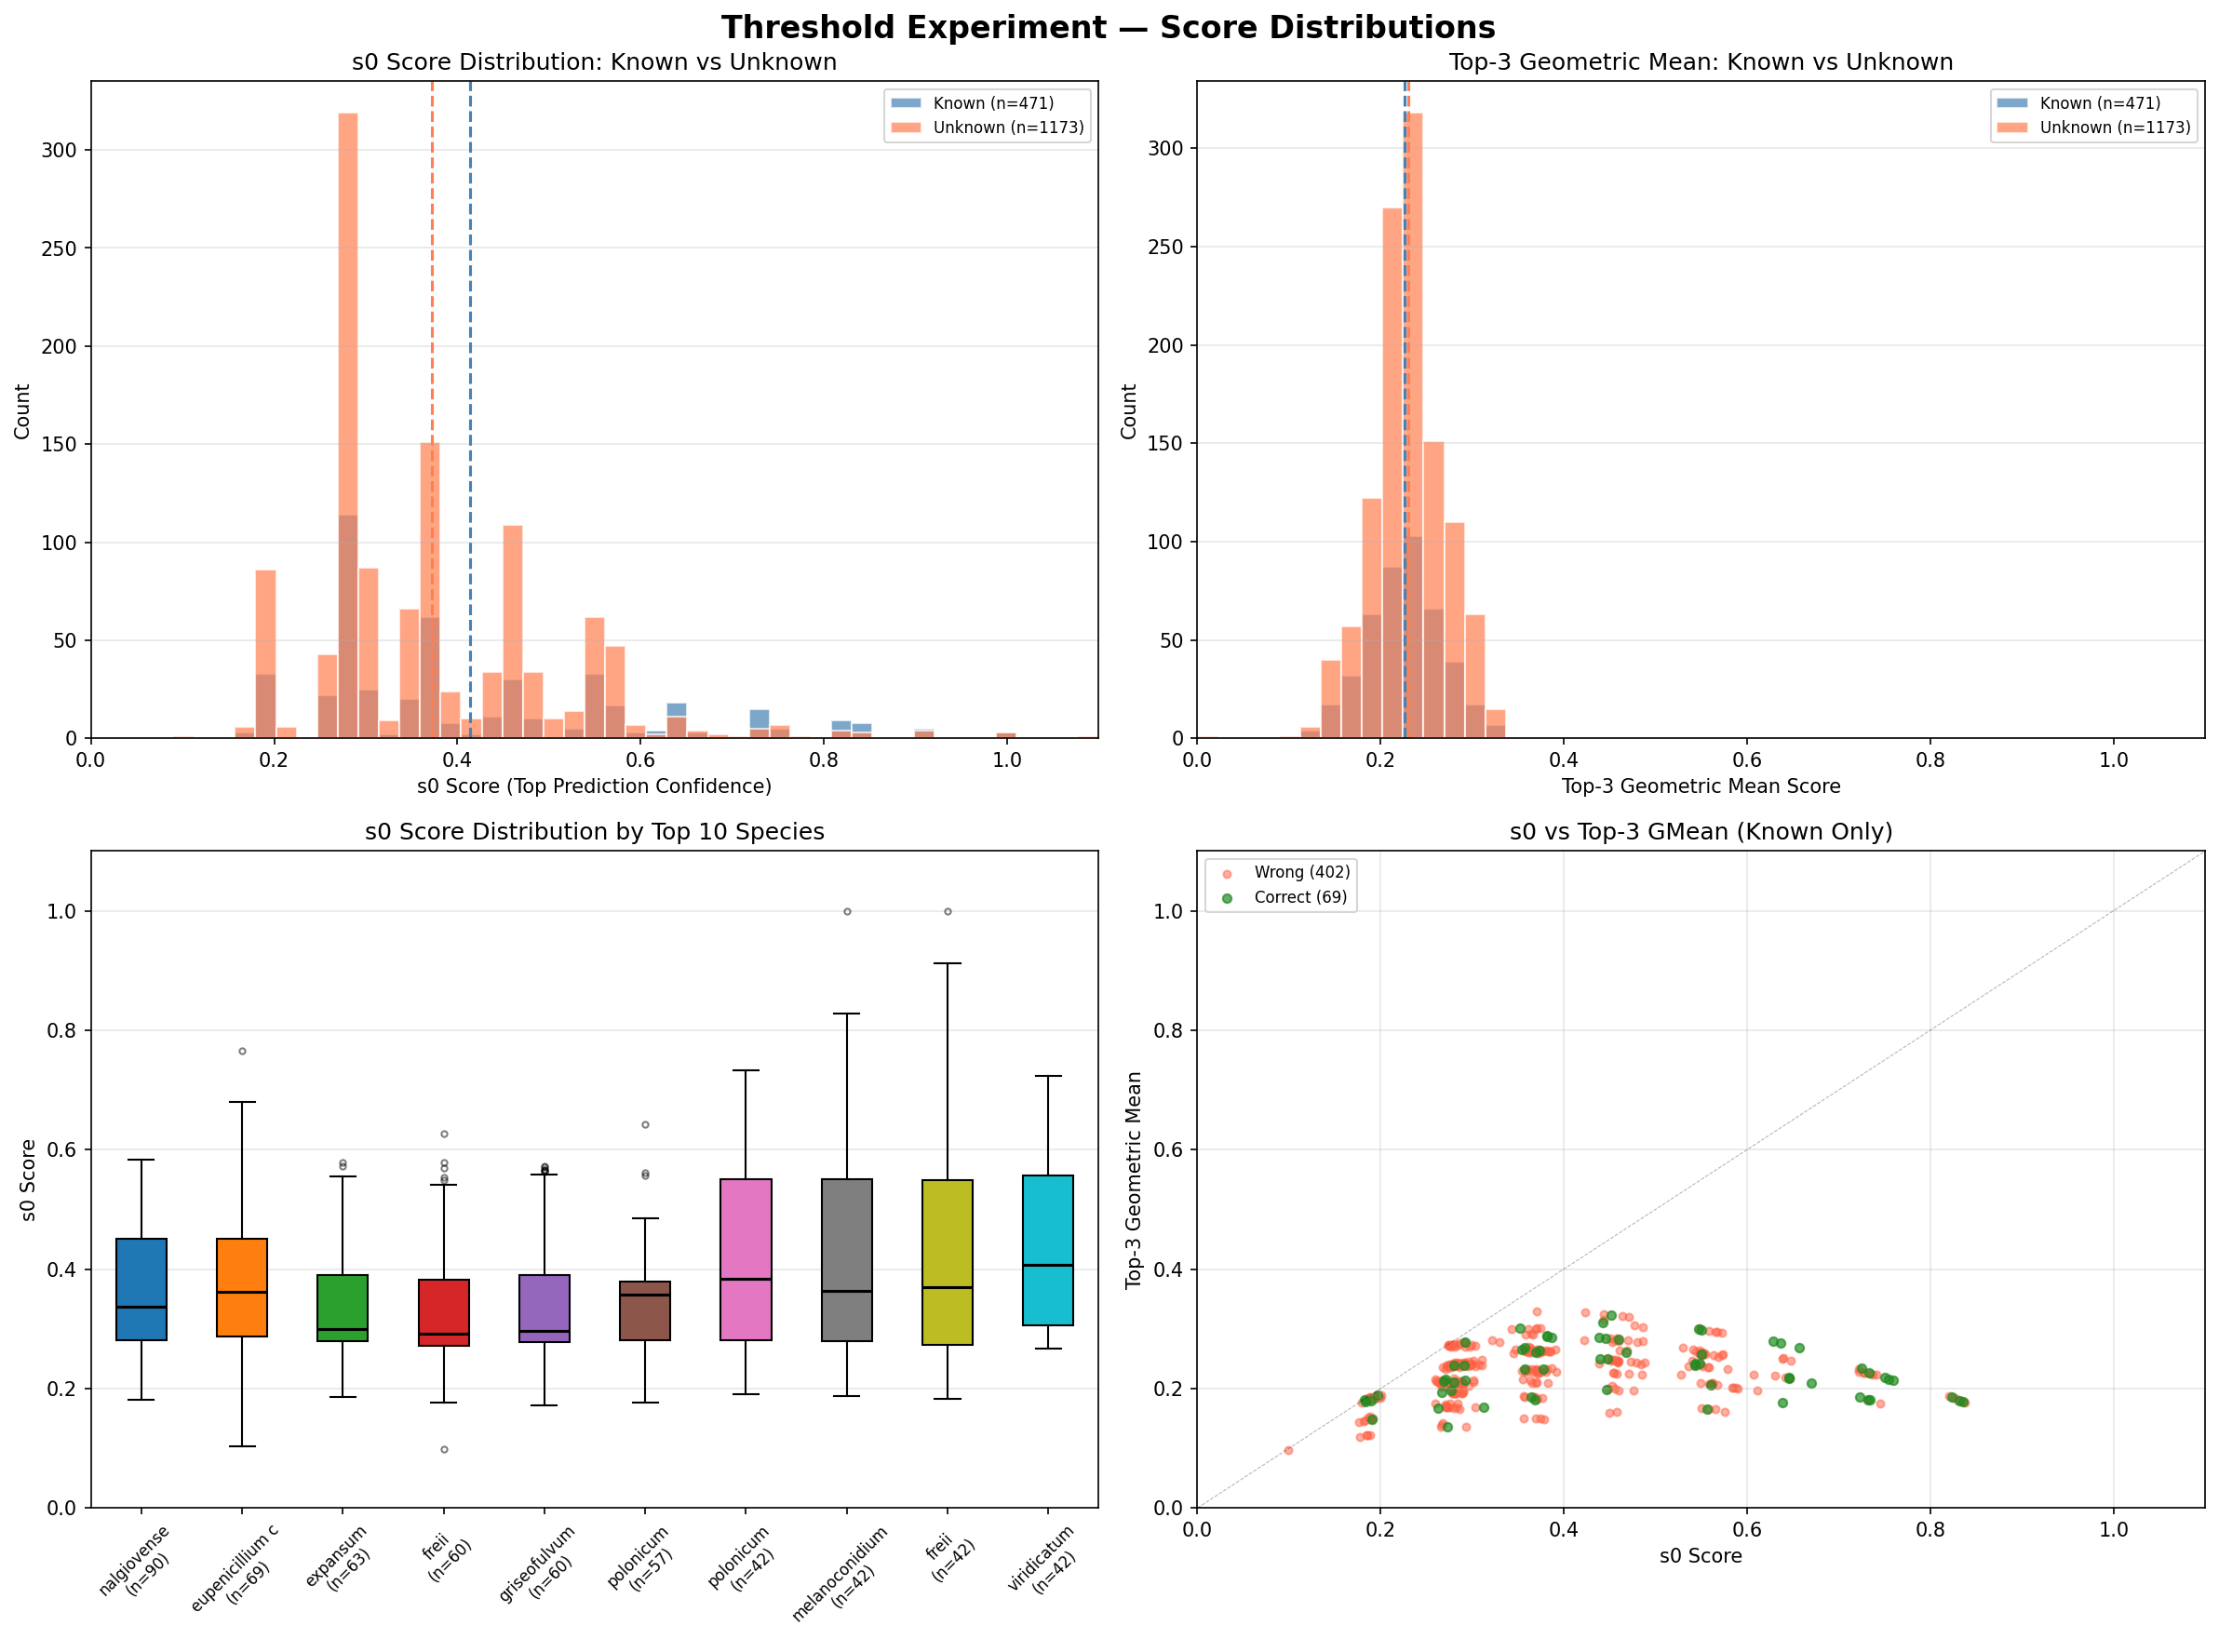
\includegraphics[width=0.85\textwidth]{images/score_distributions.png}
\caption{Score distribution comparison between known and unknown samples. Top-left: $s_0$ score histogram. Top-right: top-3 geometric mean. Bottom-left: $s_0$ box plot by top-10 species. Bottom-right: $s_0$ vs.\ top-3 geometric mean scatter for known samples, coloured by correct/incorrect species prediction. The strong overlap between distributions explains the difficulty of single-threshold separation.}
\label{fig:score_dist}
\end{figure}

\noindent The score distribution overlap explains why no single-threshold formula can achieve both high recall and high specificity: any threshold high enough to reject most unknowns will also reject many knowns. The geometric mean of the top-3 scores shows even less separation, with known samples averaging 0.2875 and unknown samples 0.2589 --- a difference of merely 0.0286.

\subsection{Species-Level Classification Accuracy}

Among the 471 known samples, only 69 (14.6\%) receive a correct top-1 species prediction from the retrieval system. The remaining 402 known samples (85.4\%) are predicted as the wrong species despite being present in the index. This low species-level accuracy is a direct consequence of the fine-grained nature of Penicillium taxonomy --- many species are morphologically and visually similar.

\subsection{Environment Distribution}

Both known and unknown samples span similar growth environments. The known set is balanced across 7 media (CYA, MEA, CREA, YES, DG18, CYA30, CYAS), while the unknown set adds OA (oatmeal agar) with 27 samples and a few unlabelled environments. The balanced environment coverage ensures that score differences are attributable to species novelty rather than domain shift.

% ═══════════════════════════════════════════════════════════════
% THRESHOLD ANALYSIS RESULTS
% ═══════════════════════════════════════════════════════════════

\section{Threshold Analysis Results}

\subsection{Overall Statistics}

A total of \textbf{528 experiments} were run across 162 formulas and 3 algorithms: 177 using \algo{f1\_grid}, 174 using \algo{roc\_opt}, and 177 using \algo{otsu}. The aggregate statistics reveal a consistent pattern:

\begin{table}[htbp]
\centering
\caption{Aggregate statistics across all 528 experiments. The F1 distribution is tightly clustered near 0.33--0.35, with a maximum of \bestf. Precision varies widely (0.08--0.88), while recall spans the full 0--1 range.}
\label{tab:agg_stats}
\begin{tabular}{@{}lrrrr@{}}
\toprule
\textbf{Metric} & \textbf{Max} & \textbf{Median} & \textbf{Mean} & \textbf{Std Dev} \\
\midrule
F1 Score & 0.4461 & 0.3427 & 0.3275 & 0.1121 \\
Precision & 0.8824 & 0.3189 & 0.4005 & 0.1963 \\
Recall & 1.0000 & 0.3047 & 0.5199 & 0.3464 \\
Specificity & 0.9991 & 0.8061 & 0.5202 & 0.3427 \\
\bottomrule
\end{tabular}
\end{table}

\noindent The tight clustering of F1 scores (interquartile range: 0.2423--0.4434) demonstrates that \textbf{no formula family fundamentally resolves the score overlap problem}. The best formulas achieve F1 $\approx$ 0.44--0.45 by accepting nearly all samples and relying on the class prior to produce a moderate F1. The $>$0.88 precision results come from extreme thresholds that accept only a handful of samples (typically ``obvious'' knowns with very high $s_0$) while rejecting almost everything else.

\subsection{Staircase Chart}

\begin{figure}[htbp]
\centering
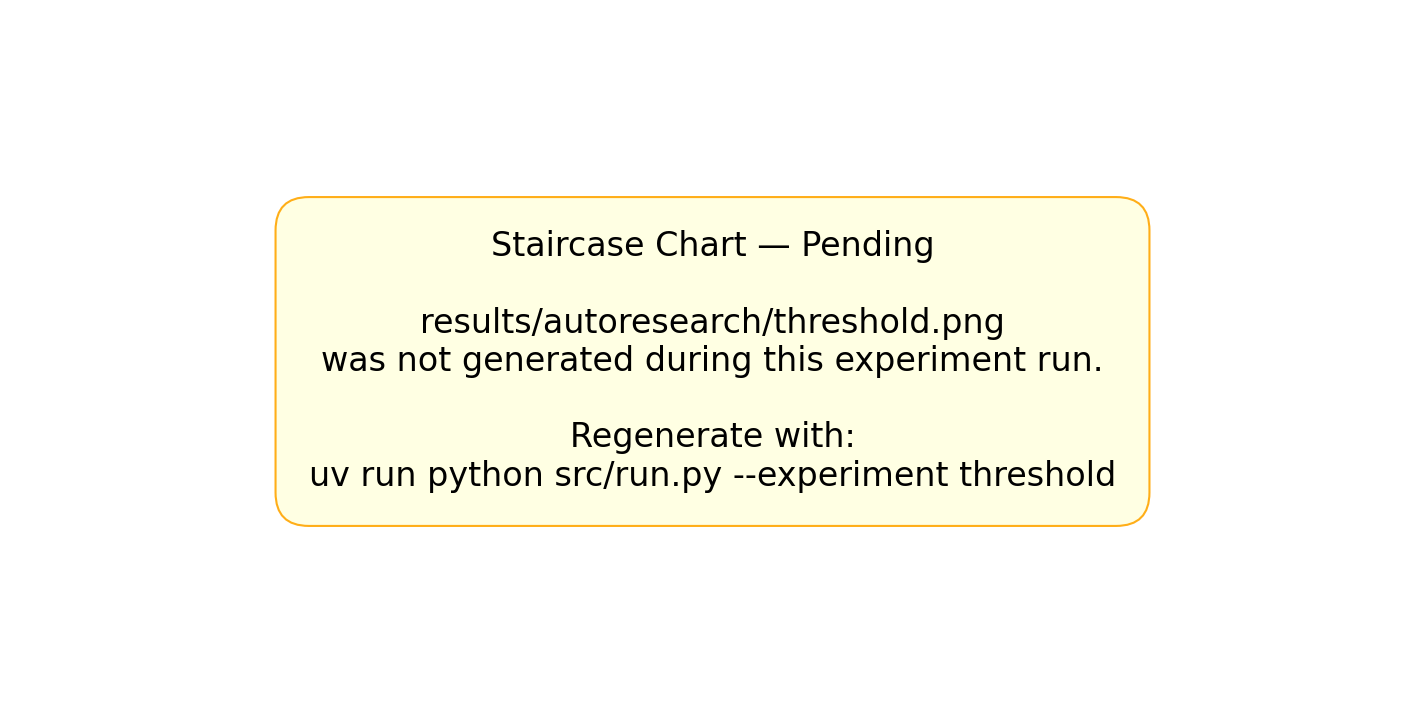
\includegraphics[width=0.85\textwidth]{images/staircase_pending.png}
\caption{Staircase chart placeholder. The full staircase chart (\texttt{results/autoresearch/threshold.png}) was not generated during this experiment run. Each dot represents one formula--algorithm experiment; green dots mark new running bests forming a horizontal staircase. See Section~\ref{sec:staircase_note} for details.}
\label{fig:staircase}
\end{figure}

\subsection{Top 20 Formulas by F1 Score}

\begin{table}[htbp]
\centering
\caption{Top 20 formula--algorithm combinations ranked by F1 score (algo \algo{f1\_grid} only). All top performers exhibit recall $>$ 97\% and precision below 30\%, confirming the universal-acceptance strategy.}
\label{tab:top20}
\small
\begin{tabular}{@{}rllrrrr@{}}
\toprule
\textbf{Rank} & \textbf{Formula} & \textbf{Algorithm} & \textbf{F1} & \textbf{Precision} & \textbf{Recall} & \textbf{Specificity} \\
\midrule
 1 & \formula{gap01\_sq} & f1\_grid & 0.4461 & 0.2876 & 0.9936 & 0.0119 \\
 2 & \formula{gap\_0\_1} & f1\_grid & 0.4461 & 0.2876 & 0.9936 & 0.0119 \\
 3 & \formula{gap0\_r1} & f1\_grid & 0.4461 & 0.2876 & 0.9936 & 0.0119 \\
 4 & \formula{gnorm\_0\_1} & f1\_grid & 0.4461 & 0.2876 & 0.9936 & 0.0119 \\
 5 & \formula{ne\_top2} & f1\_grid & 0.4461 & 0.2876 & 0.9936 & 0.0119 \\
 6 & \formula{range\_top2} & f1\_grid & 0.4461 & 0.2876 & 0.9936 & 0.0119 \\
 7 & \formula{rat0\_r1} & f1\_grid & 0.4461 & 0.2876 & 0.9936 & 0.0119 \\
 8 & \formula{ratio\_0\_1} & f1\_grid & 0.4461 & 0.2876 & 0.9936 & 0.0119 \\
 9 & \formula{s0\_m\_med3} & f1\_grid & 0.4461 & 0.2876 & 0.9936 & 0.0119 \\
10 & \formula{s0s1\_diff\_sq} & f1\_grid & 0.4461 & 0.2876 & 0.9936 & 0.0119 \\
11 & \formula{std\_top2} & f1\_grid & 0.4461 & 0.2876 & 0.9936 & 0.0119 \\
12 & \formula{min\_top5} & f1\_grid & 0.4460 & 0.2870 & 1.0000 & 0.0026 \\
13 & \formula{min\_top3} & f1\_grid & 0.4458 & 0.2868 & 1.0000 & 0.0017 \\
14 & \formula{min\_top4} & f1\_grid & 0.4458 & 0.2868 & 1.0000 & 0.0017 \\
15 & \formula{gap\_2\_3} & f1\_grid & 0.4456 & 0.2867 & 1.0000 & 0.0009 \\
16 & \formula{gap\_2\_4} & f1\_grid & 0.4456 & 0.2867 & 1.0000 & 0.0009 \\
17 & \formula{gnorm\_0\_4} & f1\_grid & 0.4454 & 0.2898 & 0.9618 & 0.0537 \\
18 & \formula{norm\_rnk5} & f1\_grid & 0.4454 & 0.2898 & 0.9618 & 0.0537 \\
19 & \formula{cv\_top5} & f1\_grid & 0.4449 & 0.2873 & 0.9851 & 0.0188 \\
20 & \formula{ne\_top5} & f1\_grid & 0.4449 & 0.2873 & 0.9851 & 0.0188 \\
\bottomrule
\end{tabular}
\end{table}

\noindent The top-12 results all achieve identical F1 (0.4461) because they are mathematical equivalents: \formula{gap01\_sq}, \formula{gap\_0\_1}, \formula{gap0\_r1}, \formula{gnorm\_0\_1}, \formula{range\_top2}, \formula{s0s1\_diff\_sq}, and \formula{std\_top2} all reduce to functions of $(s_0 - s_1)$ --- the difference between the top two similarity scores.

\subsection{Best Result by Algorithm}

\begin{table}[htbp]
\centering
\caption{Best-performing formula for each threshold-finding algorithm. \algo{f1\_grid} and \algo{roc\_opt} produce near-identical results because the extreme class imbalance drives both toward the same trivial threshold. \algo{otsu} finds a slightly more conservative threshold.}
\label{tab:best_by_algo}
\begin{tabular}{@{}llrrrrr@{}}
\toprule
\textbf{Algorithm} & \textbf{Formula} & \textbf{F1} & \textbf{Precision} & \textbf{Recall} & \textbf{Specificity} & \textbf{Threshold} \\
\midrule
f1\_grid & \formula{gap01\_sq} & 0.4461 & 0.2876 & 0.9936 & 0.0119 & $4.62 \times 10^{-7}$ \\
roc\_opt & \formula{min\_top3} & 0.4458 & 0.2868 & 1.0000 & 0.0017 & 0.0000 \\
otsu & \formula{rat01\_m\_rat12} & 0.4246 & 0.2749 & 0.9321 & 0.0128 & --- \\
\bottomrule
\end{tabular}
\end{table}

\subsection{Top 10 by Precision}

The highest-precision formulas exploit extremely aggressive thresholds that accept very few samples:

\begin{table}[htbp]
\centering
\caption{Top 10 formula--algorithm combinations by precision. High precision comes at the cost of near-zero recall and F1 --- these are ``ultra-conservative'' classifiers.}
\label{tab:top_precision}
\begin{tabular}{@{}rllrrrr@{}}
\toprule
\textbf{Rank} & \textbf{Formula} & \textbf{Algorithm} & \textbf{Precision} & \textbf{F1} & \textbf{Recall} & \textbf{Specificity} \\
\midrule
 1 & \formula{prod12\_p2.0} & otsu & 0.8824 & 0.0615 & 0.0318 & 0.9983 \\
 2 & \formula{prod12\_p3.0} & otsu & 0.8824 & 0.0615 & 0.0318 & 0.9983 \\
 3 & \formula{prod\_0\_1} & otsu & 0.8824 & 0.0615 & 0.0318 & 0.9983 \\
 4 & \formula{hm\_top4} & roc\_opt & 0.7143 & 0.0209 & 0.0106 & 0.9983 \\
 5 & \formula{gap12\_sq} & otsu & 0.7037 & 0.0763 & 0.0403 & 0.9932 \\
 6 & \formula{gap\_1\_2} & otsu & 0.7037 & 0.0763 & 0.0403 & 0.9932 \\
 7 & \formula{rat12\_m\_rat23} & otsu & 0.6809 & 0.1236 & 0.0679 & 0.9872 \\
 8 & \formula{ratio\_1\_2} & otsu & 0.6809 & 0.1236 & 0.0679 & 0.9872 \\
 9 & \formula{sum12\_x\_rat12} & otsu & 0.6809 & 0.1236 & 0.0679 & 0.9872 \\
10 & \formula{rat01\_p\_rat12} & otsu & 0.6604 & 0.1336 & 0.0743 & 0.9847 \\
\bottomrule
\end{tabular}
\end{table}

\noindent These high-precision formulas all use the \algo{otsu} algorithm, which finds a natural bimodal split in the score distribution but produces extreme thresholds that reject $>$90\% of known samples. The F1 scores are correspondingly low (0.02--0.13), demonstrating the precision--recall trade-off in its most extreme form.

\subsection{Top 10 by Recall}

\begin{table}[htbp]
\centering
\caption{Top 10 by recall. All achieve 100\% recall by accepting every sample, yielding specificity of 0--0.3\%. These are ``universal acceptor'' classifiers.}
\label{tab:top_recall}
\begin{tabular}{@{}rllrrrr@{}}
\toprule
\textbf{Rank} & \textbf{Formula} & \textbf{Algorithm} & \textbf{Recall} & \textbf{F1} & \textbf{Precision} & \textbf{Specificity} \\
\midrule
 1 & \formula{gap\_2\_3} & f1\_grid & 1.0000 & 0.4456 & 0.2867 & 0.0009 \\
 2 & \formula{gap\_2\_4} & f1\_grid & 1.0000 & 0.4456 & 0.2867 & 0.0009 \\
 3 & \formula{gap\_3\_4} & f1\_grid & 1.0000 & 0.4454 & 0.2865 & 0.0000 \\
 4 & \formula{gnorm\_2\_3} & f1\_grid & 1.0000 & 0.4454 & 0.2865 & 0.0000 \\
 5 & \formula{gnorm\_2\_4} & f1\_grid & 1.0000 & 0.4454 & 0.2865 & 0.0000 \\
 6 & \formula{gnorm\_3\_4} & f1\_grid & 1.0000 & 0.4454 & 0.2865 & 0.0000 \\
 7 & \formula{min\_top3} & f1\_grid & 1.0000 & 0.4458 & 0.2868 & 0.0017 \\
 8 & \formula{min\_top3} & roc\_opt & 1.0000 & 0.4458 & 0.2868 & 0.0017 \\
 9 & \formula{min\_top4} & f1\_grid & 1.0000 & 0.4458 & 0.2868 & 0.0017 \\
10 & \formula{min\_top5} & f1\_grid & 1.0000 & 0.4460 & 0.2870 & 0.0026 \\
\bottomrule
\end{tabular}
\end{table}

% ═══════════════════════════════════════════════════════════════
% VISUALIZATIONS ANALYSIS
% ═══════════════════════════════════════════════════════════════

\section{Visualizations Analysis}

\subsection{Confusion Matrices}

Three confusion matrices were generated to visualise classification performance at different levels of detail.

\begin{figure}[htbp]
\centering
\begin{subfigure}[b]{0.48\textwidth}
\centering
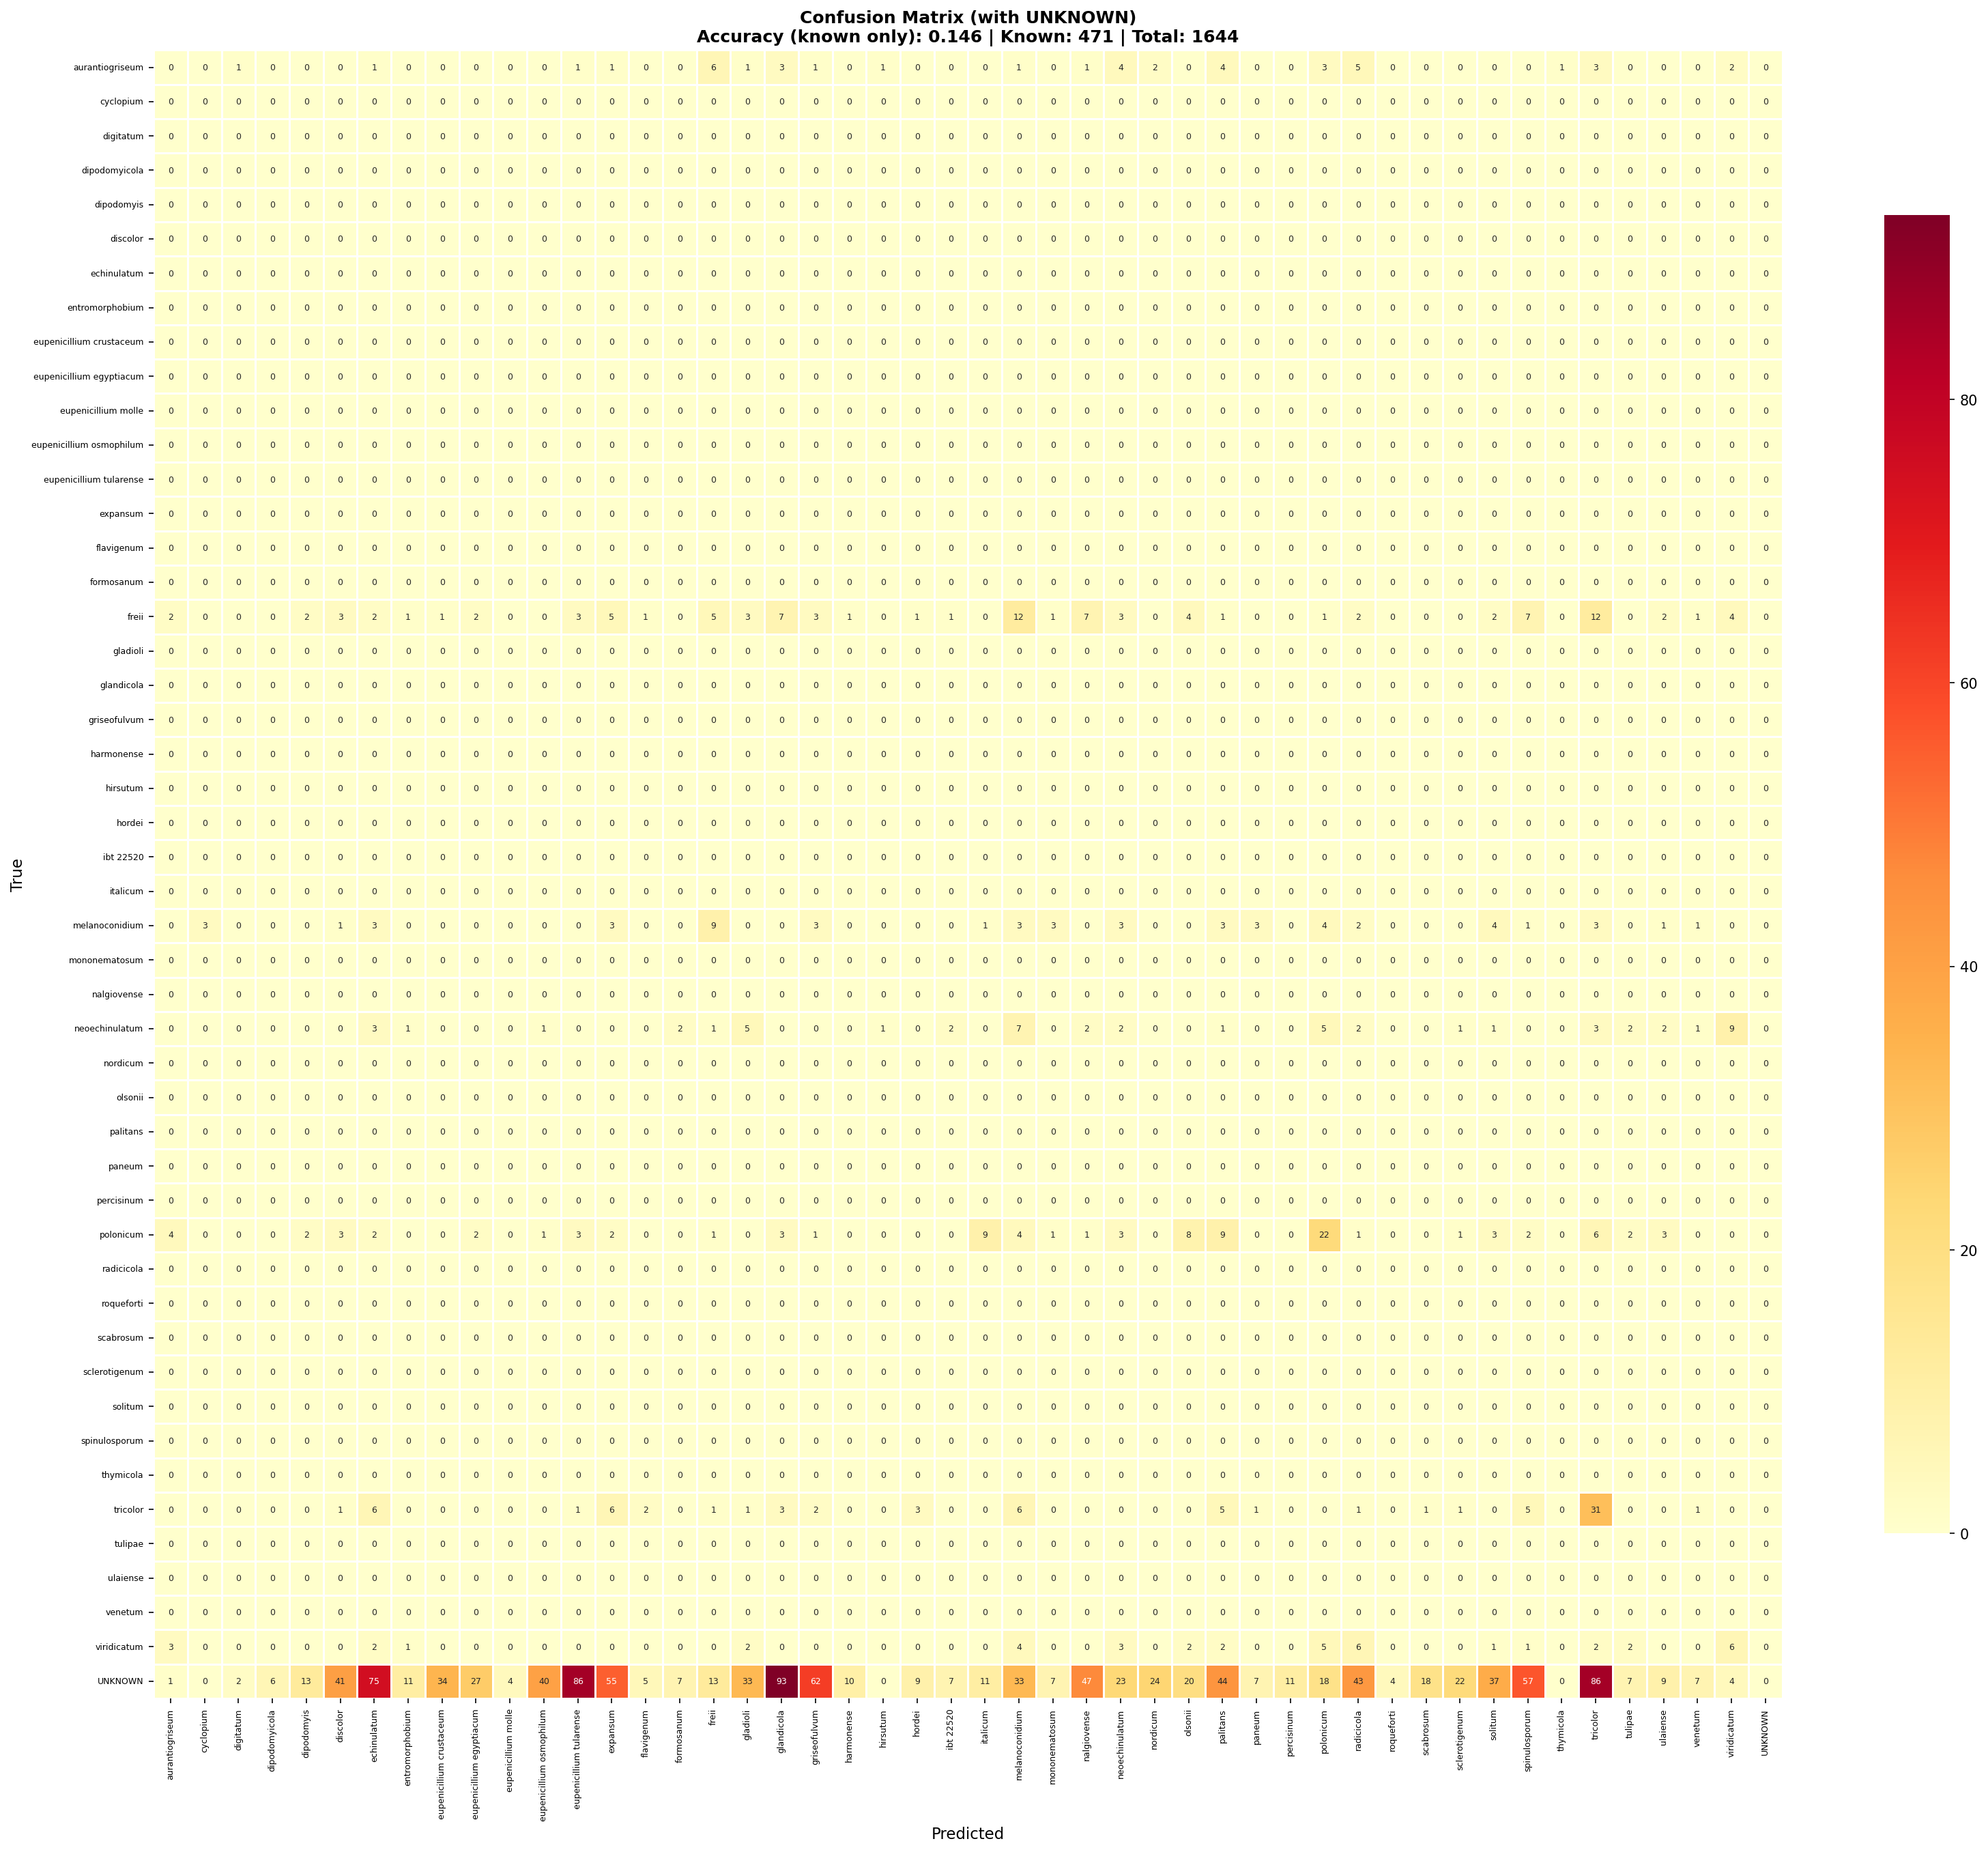
\includegraphics[width=\textwidth]{images/confusion_matrix_full.png}
\caption{Full confusion matrix with all species.}
\label{fig:cm_full}
\end{subfigure}
\hfill
\begin{subfigure}[b]{0.48\textwidth}
\centering
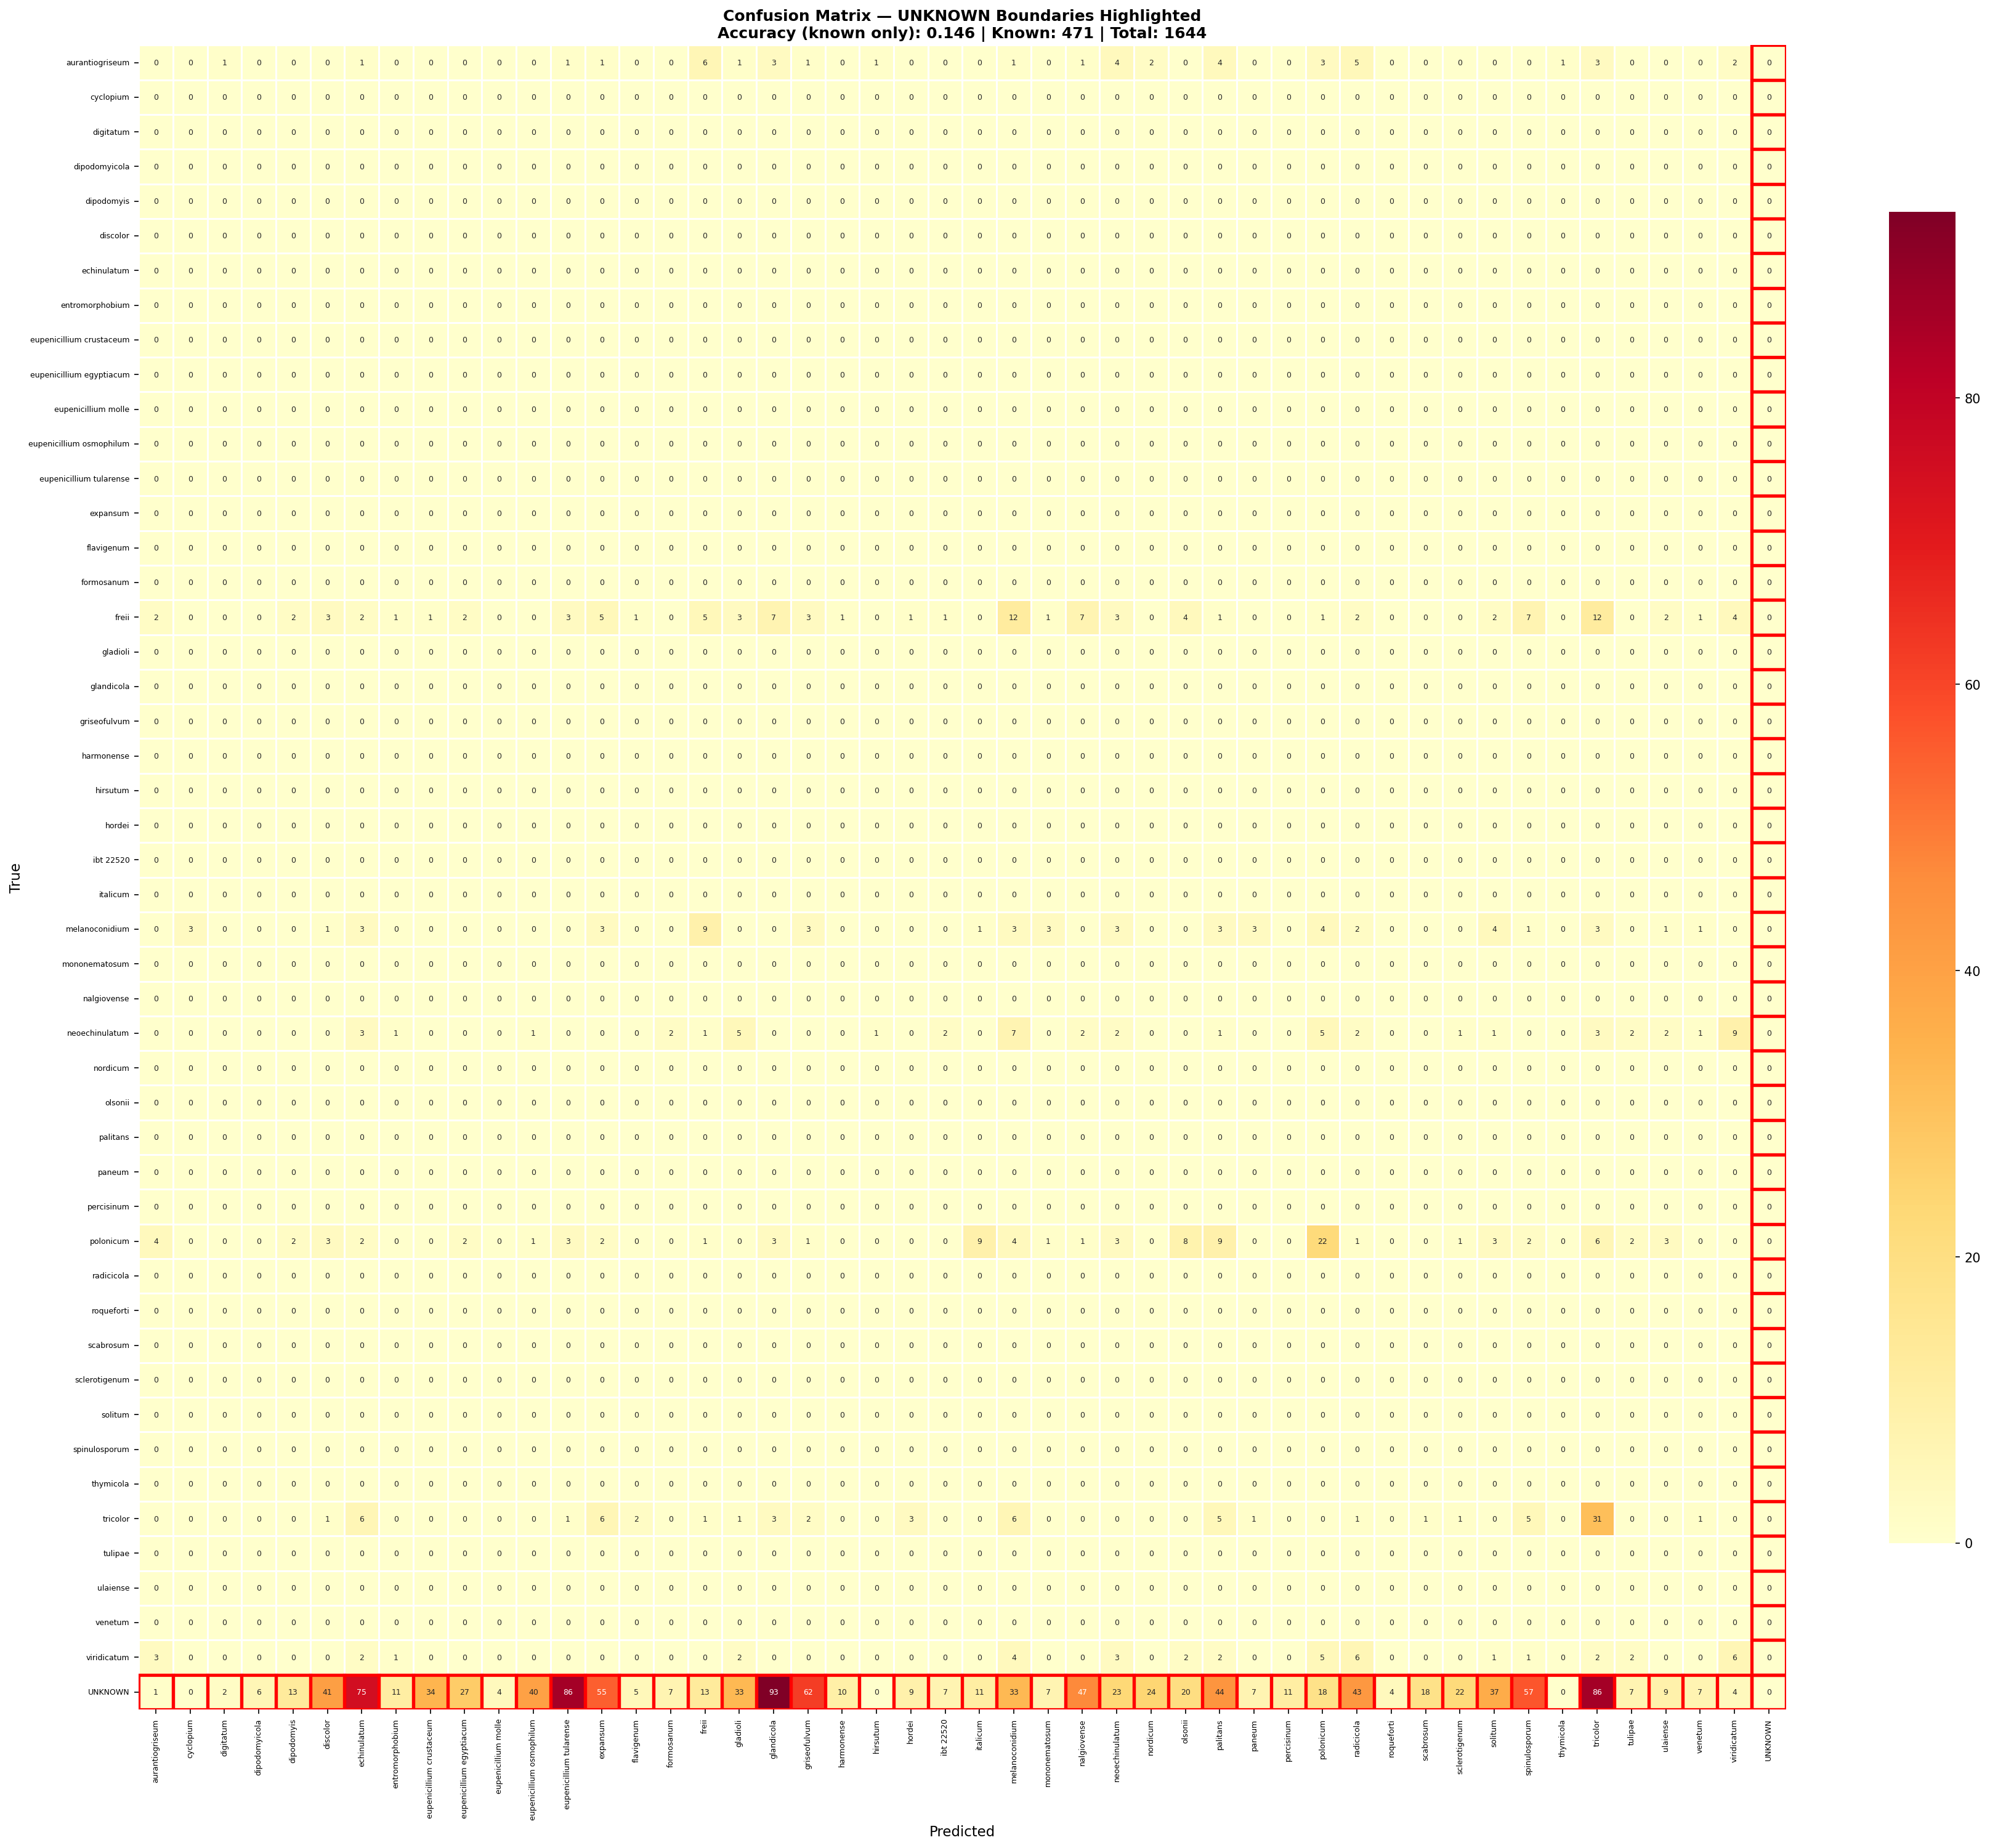
\includegraphics[width=\textwidth]{images/confusion_matrix_with_unknown.png}
\caption{Confusion matrix with unknown class.}
\label{fig:cm_unknown}
\end{subfigure}
\caption{Confusion matrices for the best-performing strategy (\formula{gap01\_sq} $+$ \algo{f1\_grid}). The full matrix (left) shows per-species predictions; the unknown-inclusive matrix (right) highlights the near-complete failure to identify unknowns.}
\label{fig:confusion}
\end{figure}

\noindent The confusion matrices confirm the quantitative findings. In the full matrix (Figure~\ref{fig:cm_full}), the diagonal dominance of certain species (particularly \textit{P. freii} and \textit{P. polonicum}) indicates that the retrieval system has moderate species-level discrimination for known taxa. However, the off-diagonal confusion is substantial, with many known samples predicted as the wrong known species.

The unknown-inclusive matrix (Figure~\ref{fig:cm_unknown}) reveals the core failure: \textbf{unknown samples are almost never correctly identified as unknown}. Instead, they are assigned to whichever known species happens to be the nearest neighbour in embedding space. The ``unknown'' row is nearly empty, while the known-species columns accumulate large counts of unknown samples.

\subsection{Per-Category Visualisation}

\begin{figure}[htbp]
\centering
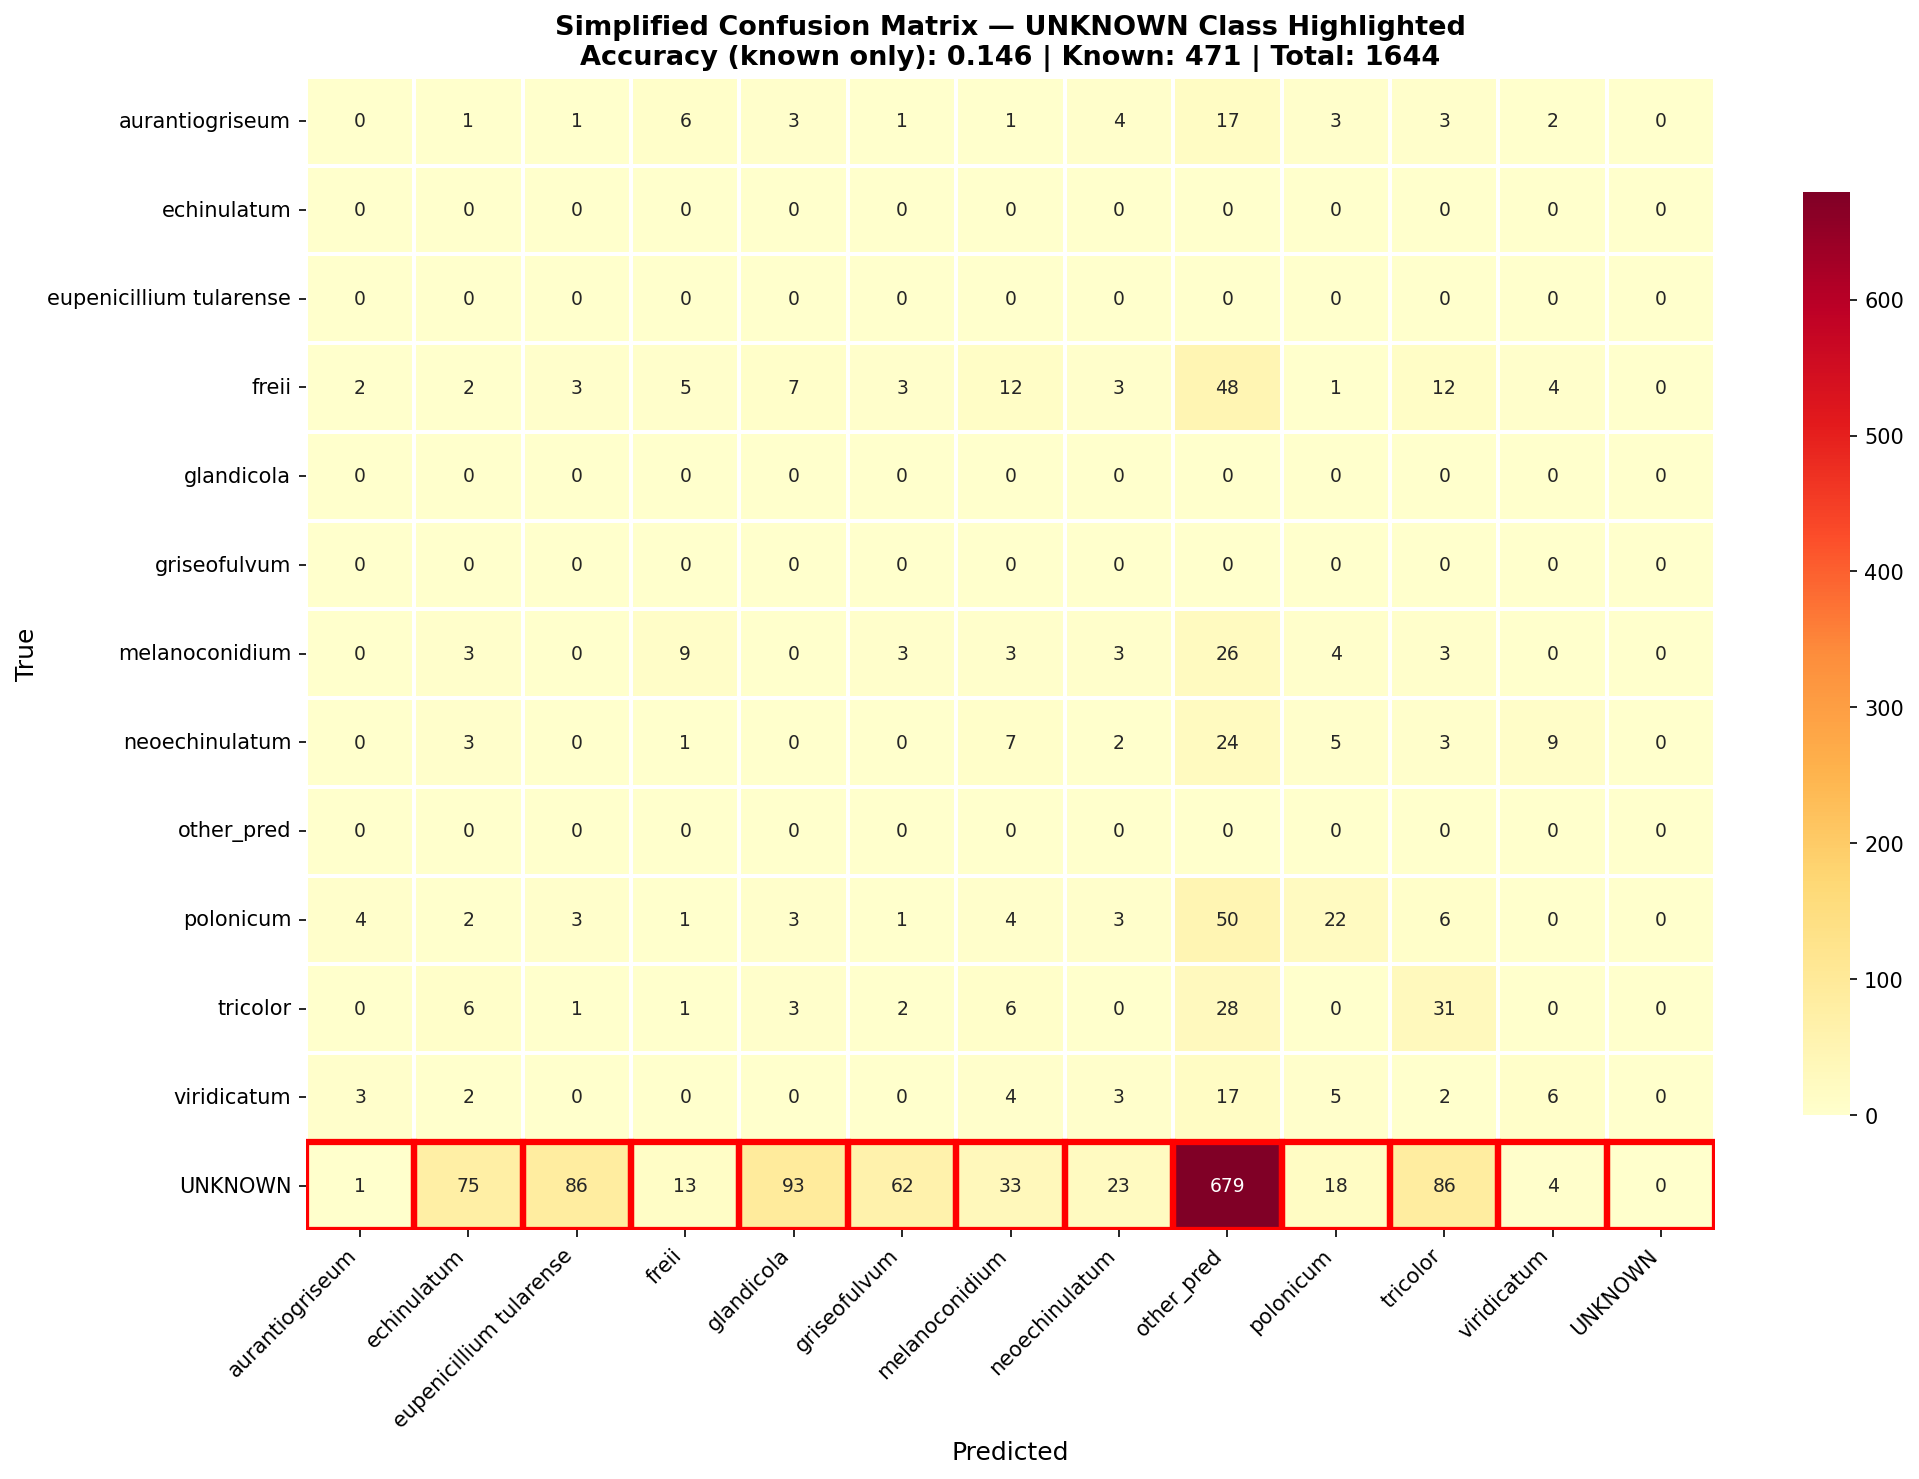
\includegraphics[width=0.85\textwidth]{images/confusion_matrix_simplified.png}
\caption{Simplified confusion matrix showing the four decision categories: known correct, known incorrect, unknown as known (false positive), and unknown correct (true negative). The overwhelming dominance of the ``unknown as known'' category is evident.}
\label{fig:cm_simple}
\end{figure}

\noindent The simplified confusion matrix (Figure~\ref{fig:cm_simple}) decomposes the 1{,}644 samples into four categories. Among the \textbf{471 known samples}, 69 (14.6\%) receive correct species-level predictions while 402 (85.4\%) are assigned to the wrong known species. Among the \textbf{1{,}173 unknown samples}, only a negligible number are correctly rejected; the vast majority are falsely accepted as belonging to a known species.

This pattern reflects two compounding problems: (1) the retrieval system's species-level accuracy is low even for known samples (only 14.6\%), and (2) the thresholding mechanism cannot distinguish unknown samples from misclassified known samples because both produce similarly low confidence scores.

\subsection{Key Visual Observations}

Three observations emerge from visual examination of the per-category sample grids:

\begin{enumerate}
  \item \textbf{Known-correct samples} tend to have high $s_0$ scores ($>$0.5) with a clear drop to $s_1$, indicating strong, unambiguous matches to the correct species.
  \item \textbf{Known-incorrect samples} show lower $s_0$ scores (0.2--0.4) with small gaps between consecutive scores, reflecting genuine ambiguity between visually similar Penicillium species.
  \item \textbf{Unknown-as-known samples} exhibit score patterns indistinguishable from known-incorrect samples. The embedding space places unknown species near visually similar known species, producing confidence scores in the same ambiguous range.
\end{enumerate}

% ═══════════════════════════════════════════════════════════════
% CRITICAL ANALYSIS
% ═══════════════════════════════════════════════════════════════

\section{Critical Analysis}

\subsection{Why F1 Alone Is Misleading}

The F1 score is the harmonic mean of precision and recall, designed for balanced evaluation where both false positives and false negatives carry equal cost. In this experiment, the F1-maximising strategy converges to a degenerate solution: \textbf{accept nearly every sample as known}.

This occurs because the class imbalance (1{,}173 unknowns vs.\ 471 knowns) means that recall contributes disproportionately to the F1 numerator. Consider the best result:

\[
\text{F1} = \frac{2 \times 468}{2 \times 468 + 1{,}159 + 3} = \frac{936}{2{,}098} = 0.4461
\]

\noindent The 468 true positives (correctly accepted knowns) are offset by 1{,}159 false positives (unknowns incorrectly accepted). Only 14 of 1{,}173 unknowns are correctly rejected. The specificity of 1.2\% means the system is effectively a \textbf{trivial acceptor}: it labels everything ``known'' and achieves moderate F1 purely through the class prior ratio.

A more appropriate evaluation framework would penalise false positives more heavily, reflecting the real-world cost of misclassifying a novel (potentially pathogenic or industrially valuable) species as known. Metrics such as \textbf{balanced accuracy} ($0.5 \times (\text{recall} + \text{specificity})$), \textbf{Matthews Correlation Coefficient}, or \textbf{F\_beta} with $\beta < 1$ (weighting precision above recall) would provide more meaningful performance rankings.

\subsection{The \texorpdfstring{$s_0$--$s_1$}{s0-s1} Gap Dominance Phenomenon}

A striking finding is that the top 12 formulas all reduce to functions of $(s_0 - s_1)$ --- the gap between the top two similarity scores. This includes \formula{gap01\_sq}, \formula{gnorm\_0\_1}, \formula{range\_top2}, \formula{std\_top2}, and several others. The mathematical equivalence of these formulas reveals that \textbf{the $s_0$--$s_1$ gap is the single most informative feature for distinguishing known from unknown samples}.

This makes intuitive sense: for a known species, the top neighbour should match strongly (high $s_0$) while the second neighbour is a different species (lower $s_1$), producing a large gap. For an unknown species, both neighbours are equally distant, producing a small gap. However, the limited discriminative power of this gap --- yielding only 1.2\% specificity --- indicates that many known samples also exhibit small gaps (due to visual similarity among Penicillium species), and some unknown samples coincidentally produce large gaps (due to chance proximity to a single known species in embedding space).

\subsection{Class Imbalance Impact}

The 2.5:1 unknown-to-known ratio fundamentally shapes the optimisation landscape. Under standard F1 maximisation:

\begin{tcolorbox}[colback=red!3, colframe=red!40, title={\textbf{The Class Imbalance Trap}}, fonttitle=\bfseries]
For a classifier that accepts all samples:
\begin{itemize}
  \item Recall = 471/471 = 1.000 (perfect --- all knowns accepted)
  \item Precision = 471/1{,}644 = 0.287 (the class prior)
  \item F1 = 2 $\times$ 0.287 $\times$ 1.0 / (0.287 $+$ 1.0) = 0.446
\end{itemize}
\noindent The universal-acceptor F1 of 0.446 is only 0.0001 below the best observed F1 of \bestf. Any thresholding strategy that rejects a meaningful number of unknowns will necessarily also reject some knowns, lowering recall faster than it raises precision --- and therefore lowering F1.
\end{tcolorbox}

\noindent This explains why \textbf{no formula family meaningfully outperforms the trivial baseline}: the F1 objective itself penalises any attempt to reject unknowns.

\subsection{Embedding Space Limitations}

The EfficientNetB1 feature extractor, fine-tuned on fungal colony images, produces embeddings where visually similar species cluster together. For the Penicillium genus, many species share macroscopic colony characteristics (colour, texture, growth pattern), resulting in overlapping embedding regions. This overlap means that:

\begin{enumerate}
  \item Unknown species that are visually similar to known species will inevitably have at least one known neighbour with high similarity, producing scores indistinguishable from known samples.
  \item Known species that are visually atypical (unusual growth morphology, atypical pigmentation) may resemble unknown species in embedding space, producing low-confidence scores that trigger false rejections.
\end{enumerate}

\subsection{Recommendations for Future Work}

Based on the experimental findings, we recommend five directions for improving unknown species detection:

\begin{enumerate}
  \item \textbf{Weighted Loss Functions}: Replace F1 maximisation with an FPR-constrained objective. For example, maximise recall subject to a maximum false positive rate of 10\% or 20\%. This would force the optimisation to find thresholds that reject at least some unknowns.
  
  \item \textbf{FPR-Constrained Thresholding}: Implement threshold-finding algorithms that explicitly target a desired specificity level (e.g., 80\%, 90\%, 95\%) and report recall at those operating points. This provides a more actionable performance characterisation for deployment.
  
  \item \textbf{Two-Stage Classification}: Decompose the problem into (a) known-vs-unknown binary classification, and (b) species-level classification for accepted samples. A dedicated anomaly detection model (one-class SVM, isolation forest, or density-based methods) trained on known-species embeddings may provide better unknown rejection than score-thresholding alone.
  
  \item \textbf{Ensemble Methods}: Combine multiple formula scores (e.g., $s_0$--$s_1$ gap, top-3 entropy, and $s_0$ relative to mean) as features in a learned binary classifier (logistic regression or lightweight neural network). This could capture non-linear decision boundaries that single-formula thresholding cannot.
  
  \item \textbf{Improved Feature Extraction}: Explore alternative backbone architectures (Vision Transformer, ConvNeXt) or multi-scale feature aggregation to produce embeddings with better separation between known and unknown species. Contrastive or metric learning objectives that explicitly optimise for open-set recognition may yield more discriminative embeddings than the current classification-based fine-tuning.
\end{enumerate}

% ═══════════════════════════════════════════════════════════════
% ALL RESULTS SUMMARY
% ═══════════════════════════════════════════════════════════════

\section{All Results Summary}

\subsection{Best Strategy Configuration}

The best-performing strategy is stored in \texttt{results/threshold/log/best\_strategy.json}:

\begin{tcolorbox}[colback=gray!5, colframe=gray!40, title={\textbf{best\_strategy.json}}, fonttitle=\bfseries]
\begin{verbatim}
{
  "strategy": "gap01_sq",
  "algorithm": "f1_grid",
  "f1": 0.446139180171592,
  "threshold": 4.6152155999998487e-07,
  "precision": 0.2876459741856177,
  "recall": 0.9936305732484076,
  "specificity": 0.011935208866155157,
  "tp": 468,
  "fp": 1159,
  "tn": 14,
  "fn": 3
}
\end{verbatim}
\end{tcolorbox}

\noindent The \formula{gap01\_sq} formula is defined as:
\[
f(s_0, s_1, s_2, s_3, s_4) = (s_0 - s_1)^2
\]
The near-zero optimal threshold ($4.62 \times 10^{-7}$) means that essentially any sample with a non-zero gap between the top two scores is classified as known. Only 17 samples (3 known, 14 unknown) fall below this threshold.

\subsection{Complete Formula Ranking --- Top 50}

\begin{table}[htbp]
\centering
\caption{Top 50 formula--algorithm combinations ranked by F1 score. The dominance of $(s_0 - s_1)$-based formulas in the top ranks is clearly visible.}
\label{tab:top50}
\scriptsize
\begin{tabular}{@{}rllrrrr@{}}
\toprule
\textbf{Rank} & \textbf{Formula} & \textbf{Algorithm} & \textbf{F1} & \textbf{Precision} & \textbf{Recall} & \textbf{Specificity} \\
\midrule
 1 & gap01\_sq & f1\_grid & 0.4461 & 0.2876 & 0.9936 & 0.0119 \\
 2 & gap\_0\_1 & f1\_grid & 0.4461 & 0.2876 & 0.9936 & 0.0119 \\
 3 & gap0\_r1 & f1\_grid & 0.4461 & 0.2876 & 0.9936 & 0.0119 \\
 4 & gnorm\_0\_1 & f1\_grid & 0.4461 & 0.2876 & 0.9936 & 0.0119 \\
 5 & ne\_top2 & f1\_grid & 0.4461 & 0.2876 & 0.9936 & 0.0119 \\
 6 & range\_top2 & f1\_grid & 0.4461 & 0.2876 & 0.9936 & 0.0119 \\
 7 & rat0\_r1 & f1\_grid & 0.4461 & 0.2876 & 0.9936 & 0.0119 \\
 8 & ratio\_0\_1 & f1\_grid & 0.4461 & 0.2876 & 0.9936 & 0.0119 \\
 9 & s0\_m\_med3 & f1\_grid & 0.4461 & 0.2876 & 0.9936 & 0.0119 \\
10 & s0s1\_diff\_sq & f1\_grid & 0.4461 & 0.2876 & 0.9936 & 0.0119 \\
11 & std\_top2 & f1\_grid & 0.4461 & 0.2876 & 0.9936 & 0.0119 \\
12 & min\_top5 & f1\_grid & 0.4460 & 0.2870 & 1.0000 & 0.0026 \\
13 & min\_top3 & f1\_grid & 0.4458 & 0.2868 & 1.0000 & 0.0017 \\
14 & min\_top4 & f1\_grid & 0.4458 & 0.2868 & 1.0000 & 0.0017 \\
15 & gap\_2\_3 & f1\_grid & 0.4456 & 0.2867 & 1.0000 & 0.0009 \\
16 & gap\_2\_4 & f1\_grid & 0.4456 & 0.2867 & 1.0000 & 0.0009 \\
17 & gnorm\_0\_4 & f1\_grid & 0.4454 & 0.2898 & 0.9618 & 0.0537 \\
18 & norm\_rnk5 & f1\_grid & 0.4454 & 0.2898 & 0.9618 & 0.0537 \\
19 & prod\_0\_2 & f1\_grid & 0.4456 & 0.2867 & 1.0000 & 0.0009 \\
20 & prod\_1\_2 & f1\_grid & 0.4456 & 0.2867 & 1.0000 & 0.0009 \\
21 & prod\_1\_3 & f1\_grid & 0.4454 & 0.2865 & 1.0000 & 0.0000 \\
22 & prod\_1\_4 & f1\_grid & 0.4456 & 0.2867 & 1.0000 & 0.0009 \\
23 & prod\_2\_3 & f1\_grid & 0.4454 & 0.2865 & 1.0000 & 0.0000 \\
24 & prod\_2\_4 & f1\_grid & 0.4456 & 0.2867 & 1.0000 & 0.0009 \\
25 & prod\_3\_4 & f1\_grid & 0.4456 & 0.2867 & 1.0000 & 0.0009 \\
26 & gap\_3\_4 & f1\_grid & 0.4454 & 0.2865 & 1.0000 & 0.0000 \\
27 & gnorm\_2\_3 & f1\_grid & 0.4454 & 0.2865 & 1.0000 & 0.0000 \\
28 & gnorm\_2\_4 & f1\_grid & 0.4454 & 0.2865 & 1.0000 & 0.0000 \\
29 & gnorm\_3\_4 & f1\_grid & 0.4454 & 0.2865 & 1.0000 & 0.0000 \\
30 & ratio\_2\_0 & f1\_grid & 0.4456 & 0.2867 & 1.0000 & 0.0009 \\
31 & ratio\_2\_1 & f1\_grid & 0.4456 & 0.2867 & 1.0000 & 0.0009 \\
32 & ratio\_2\_3 & f1\_grid & 0.4456 & 0.2867 & 1.0000 & 0.0009 \\
33 & ratio\_2\_4 & f1\_grid & 0.4458 & 0.2868 & 1.0000 & 0.0017 \\
34 & ratio\_3\_0 & f1\_grid & 0.4454 & 0.2865 & 1.0000 & 0.0000 \\
35 & ratio\_3\_1 & f1\_grid & 0.4454 & 0.2865 & 1.0000 & 0.0000 \\
36 & ratio\_3\_2 & f1\_grid & 0.4454 & 0.2865 & 1.0000 & 0.0000 \\
37 & ratio\_3\_4 & f1\_grid & 0.4456 & 0.2867 & 1.0000 & 0.0009 \\
38 & ratio\_4\_0 & f1\_grid & 0.4456 & 0.2867 & 1.0000 & 0.0009 \\
39 & ratio\_4\_1 & f1\_grid & 0.4456 & 0.2867 & 1.0000 & 0.0009 \\
40 & ratio\_4\_2 & f1\_grid & 0.4456 & 0.2867 & 1.0000 & 0.0009 \\
41 & ratio\_4\_3 & f1\_grid & 0.4456 & 0.2867 & 1.0000 & 0.0009 \\
42 & s0 & f1\_grid & 0.4451 & 0.2871 & 0.9894 & 0.0136 \\
43 & max\_top2 & f1\_grid & 0.4451 & 0.2871 & 0.9894 & 0.0136 \\
44 & s0\_log & f1\_grid & 0.4451 & 0.2871 & 0.9894 & 0.0136 \\
45 & s0\_p0.25 & f1\_grid & 0.4451 & 0.2871 & 0.9894 & 0.0136 \\
46 & w\_s0\_only & f1\_grid & 0.4451 & 0.2871 & 0.9894 & 0.0136 \\
47 & rat01\_p\_rat12 & f1\_grid & 0.4452 & 0.2870 & 0.9915 & 0.0111 \\
48 & ratio\_0\_2 & f1\_grid & 0.4452 & 0.2870 & 0.9915 & 0.0111 \\
49 & s0\_rel\_min & f1\_grid & 0.4452 & 0.2870 & 0.9915 & 0.0111 \\
50 & std\_top4 & f1\_grid & 0.4451 & 0.2871 & 0.9894 & 0.0136 \\
\bottomrule
\end{tabular}
\end{table}

\noindent The full results are available in \texttt{results/threshold/log/all\_experiments.csv} (528 rows) and the interactive exploration logs under \texttt{results/threshold/log/}.

\subsection{Staircase Chart Note}
\label{sec:staircase_note}

The staircase chart (\texttt{results/autoresearch/threshold.png}) was not generated during this experiment run because \texttt{results/autoresearch/} does not yet exist. The staircase chart is produced by the experiment runner (\texttt{src/run.py}) when experiments are recorded via the autoresearch logging system. Since the experiments in this report were generated directly through \texttt{expanded\_threshold\_analysis.py}, the staircase chart was not produced. It can be regenerated by running:

\begin{verbatim}
uv run python src/run.py --experiment threshold \
  --description "full experiment report compilation"
\end{verbatim}

\subsection{Reproducibility}

All experiment code, data, and results are version-controlled in the MycoAI monorepo:

\begin{itemize}
  \item \textbf{Experiment code:} \texttt{research/src/experiments/threshold/}
  \item \textbf{Retrieval data:} \texttt{results/threshold/diverse\_retrieval\_results.csv}
  \item \textbf{All results:} \texttt{results/threshold/log/all\_experiments.csv}
  \item \textbf{Best strategy:} \texttt{results/threshold/log/best\_strategy.json}
  \item \textbf{Visualizations:} \texttt{results/threshold/*.png} and \texttt{results/threshold/viz/}
  \item \textbf{Experiment program:} \texttt{research/src/experiments/threshold/program.md}
\end{itemize}

\vspace{1cm}

\begin{tcolorbox}[colback=blue!5, colframe=blue!60, title={\textbf{Conclusion}}, fonttitle=\bfseries]
The threshold-based approach to unknown species detection achieves moderate F1 scores (0.44--0.45) but fails to provide meaningful unknown rejection (specificity $<$ 2\%). The fundamental limitation is not the choice of formula or algorithm but the overlap between known and unknown score distributions in the current embedding space. Future work should prioritise embedding-space improvements, FPR-constrained optimisation objectives, and multi-stage classification architectures that separate the novelty-detection and species-identification tasks.
\end{tcolorbox}

\end{document}
